
\subsection{Structural vs. behavioral} \label{sec:structuralOrBehavioralImplementation}
%As mentioned in section \ref{structuralOrBehavioral}, it is difficult to draw a reliable diagram with components and wires when implementing a behavioral design. However: the computations done by the Co-P resemble those performed by the customized processor in A2 which was implemented structurally, so we can sketch a plausible diagram.\\

As mentioned in section \ref{sec:structuralOrBehavioralDesign}, the Co-P is designed behaviorally, meaning there is no exact diagram showing how components are combined. However, using the structure for the CPU we can generalize such a structure, by altering the \texttt{SHUTTLE}. The \texttt{SHUTTLE} now handles interaction with both the BUS and the direct link between CPU and Co-P. Meaning this structure is a template for both CPU and Co-P even if the Co-P is linked directly or on the BUS (with the latter not using the direct link). The structure is shown in figure \ref{fig:GeneralStructure}.

\begin{figure}[H]
    \centering
    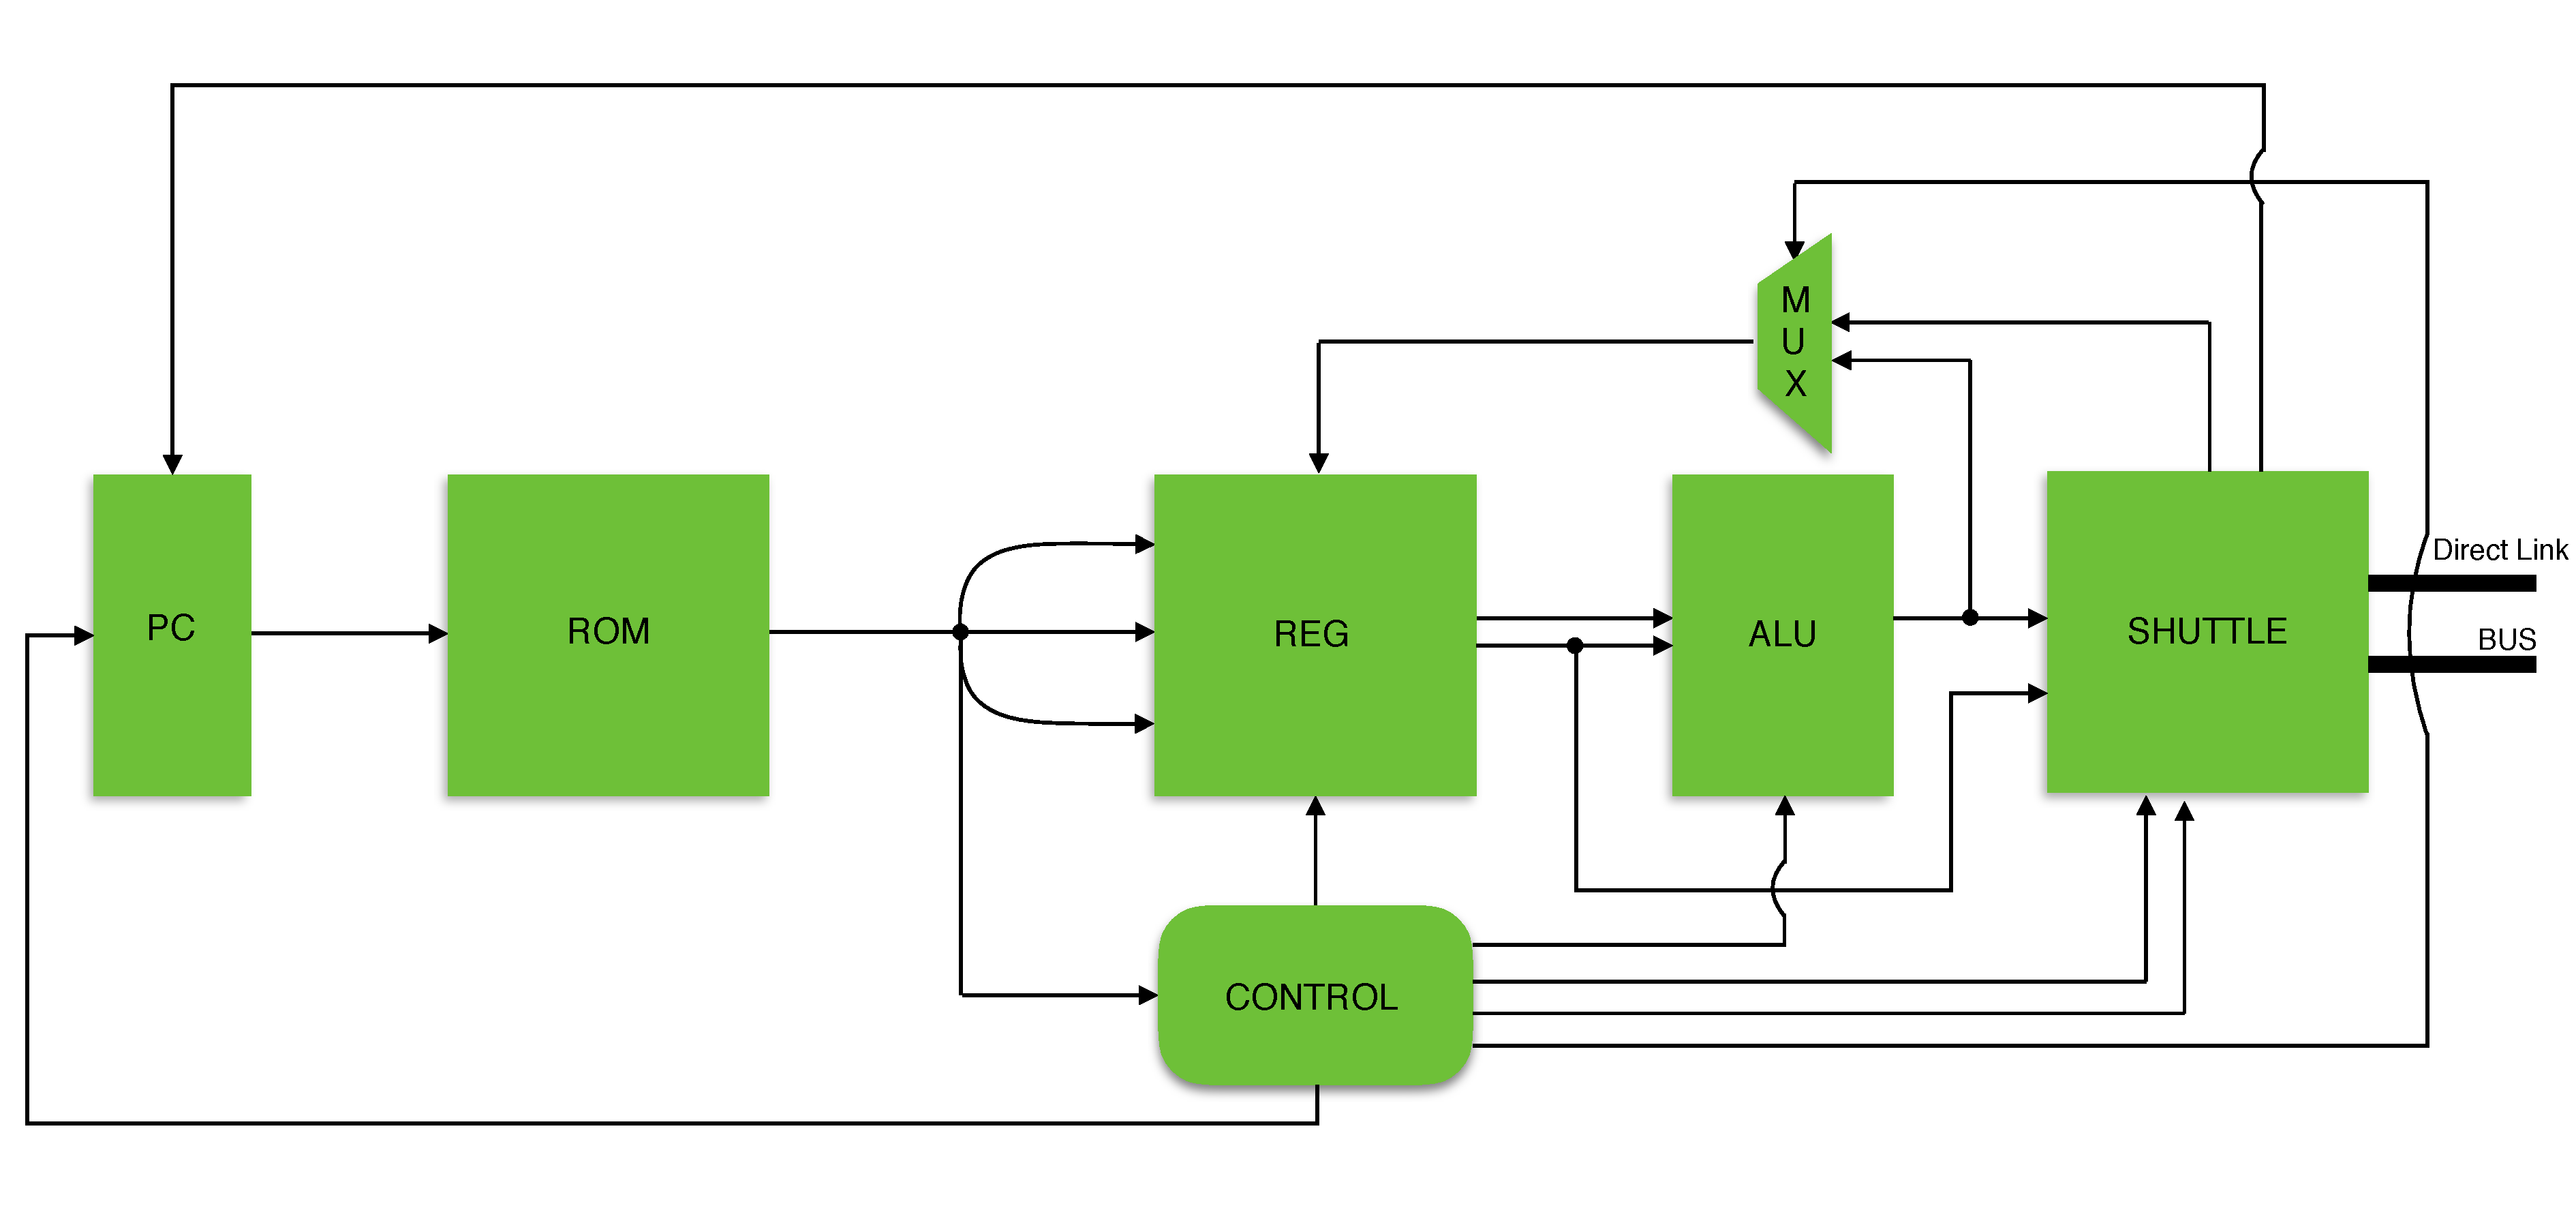
\includegraphics[width = \textwidth]{2Implementation/fig/ComputerArchitecture_A3}
    \caption{General structure for CPU or Co-P.}
    \label{fig:GeneralStructure}
\end{figure}

However, since the Co-P is designed behaviorally, the algorithm is more precisely sketched by the following fsm flowcharts.

\subsection{Solution 1: Co-P on the BUS}\label{sec:implementation1}

The design of the Co-P is viewed in the fsm flowchart in figure \ref{fig:fsm1}. 

\begin{figure}[H]
    \centering
    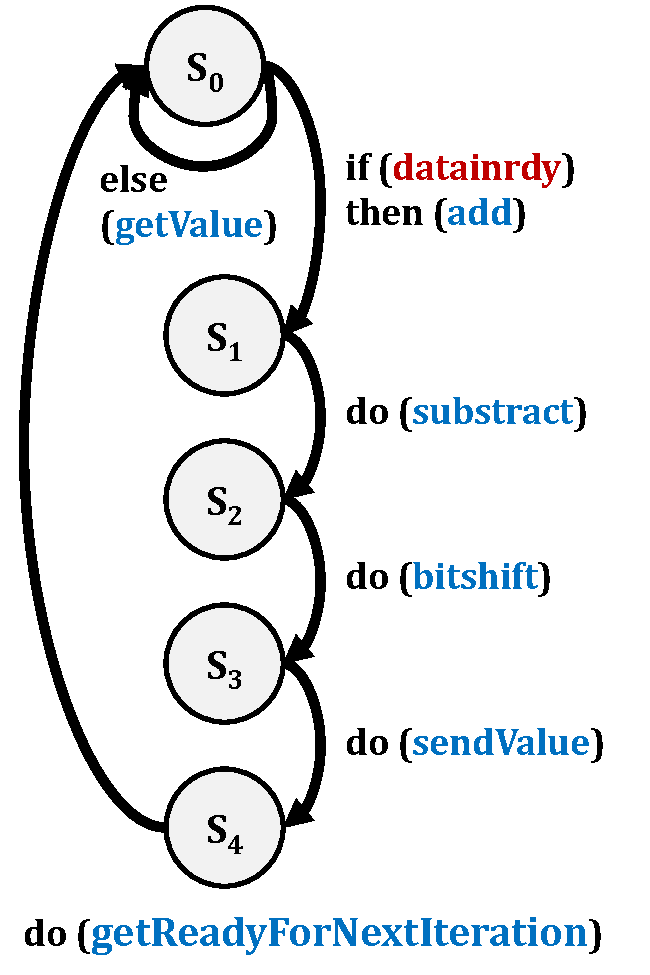
\includegraphics[width=0.45\textwidth]{2Implementation/fig/fsm1.pdf}
    \caption{FSM flowchart for the Co-P in solution 1, Co-P on the bus.}
    \label{fig:fsm1}
\end{figure}


Rough overview of \underline{s}ignal \underline{f}low \underline{g}raphs (\textbf{sfg}s): 
\begin{itemize}
\item \texttt{getValue}: Co-P gets a new data point from the CPU through the bus, and stores it in a register: \texttt{datainr = datain}. Co-P sets \texttt{dataoutrdyr = 0}, signalling that the result has not yet been processed. If the CPU did not send a value this cycle, then \texttt{datainrdy == 0}, and Co-P keeps performing \texttt{getValue}.

\item \texttt{add}: If \texttt{datainrdy == 1}, Co-P adds the new value to the register containing the sum of the previous 32 data points: \texttt{SUMr = SUMr + datainr}.

\item \texttt{subtract}: Co-P subtracts the last data value from the sum: \texttt{SUMr = SUMr - C31}.

\item \texttt{bitshift}: Divides the sum by 32 by bitshifting: \texttt{dataoutr = SUMr >> 5}.

\item \texttt{sendValue}: Sets \texttt{dataoutrdyr = 1}, signalling the BUS that the result is ready. The BUS sends the result to CPU.

\item \texttt{getReadyForNextIteration}: Co-P updates the 32 registers keeping track of the last 32 elements. The first register value is set to the new data point, \texttt{C00 = datainr}, while the other 31 registers are shifted, following pattern $C_n = C_{n-1}$, i.e. \texttt{C01 = C00}, ..., \texttt{C31 = C30}. 
\end{itemize}

\newpage
\subsection{Solution 2: Co-P linked directly to CPU}

The design of the Co-P is viewed on the fsm flowchart in figure \ref{fig:fsm2}. 

\begin{figure}[H]
    \centering
    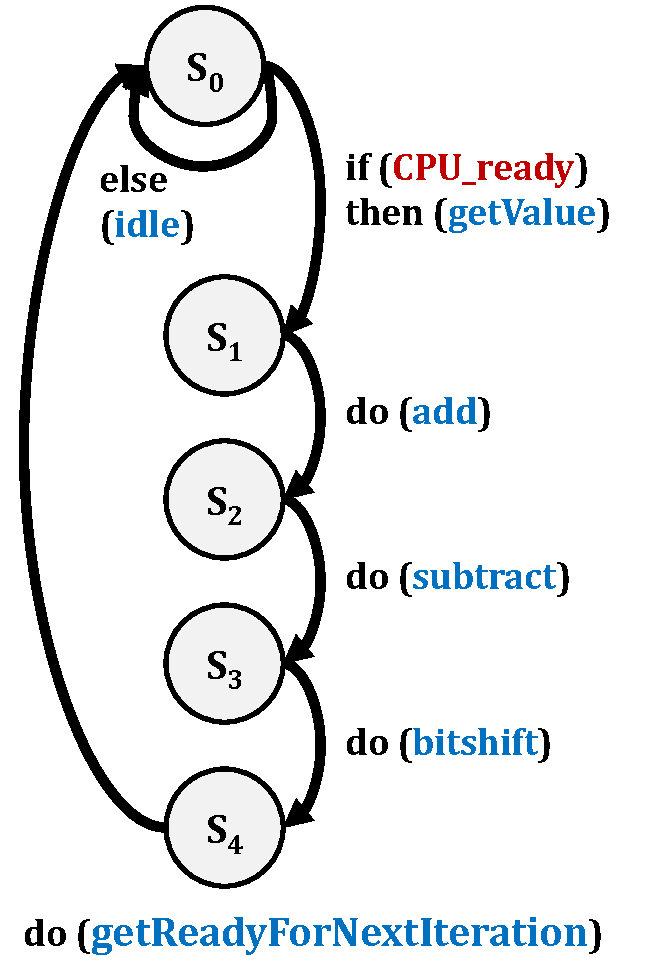
\includegraphics[width=0.45\textwidth]{2Implementation/fig/fsm2.pdf}
    \caption{FSM flowchart for the Co-P in solution 2, Co-P linked directly to CPU.}
    \label{fig:fsm2}
\end{figure}

Rough overview of \underline{s}ignal \underline{f}low \underline{g}raphs (\textbf{sfg}s): 
\begin{itemize}
\item \texttt{idle}: If the Co-P is not currently computing the filter, it stays idle, updating its register \texttt{CO\_readyr = 1}, flagging to the CPU that Co-P is ready for a handshake.

\item \texttt{getValue}: If \texttt{CPU\_ready == 1}, the Co-P performs the data swap and begins its chain of computations. This \texttt{getValue} sfg is similar to the one in solution 1, except the Co-P receives data directly from the CPU, not waiting for the BUS. 

\item \texttt{add, subtract, bitshift}: Identical to the sfgs in solution 1.

\item \texttt{getReadyForNextIteration}: As in solution 1, Co-P updates the 32 registers keeping track of the last 32 elements. 
\end{itemize}

\textbf{Interaction between Co-P and CPU:} Notice that solution 2 does not have an sfg \texttt{sendValue}. Instead, when Co-P is done with its chain of computations, it returns to \texttt{idle}, setting \texttt{CO\_readyr = 1}. \\

This register thus has a double use: it means that the Co-P is ready for a new value from the CPU, \textit{and} that the Co-P is done with its previous computation.

\subsection{Interaction patterns}

\textbf{Approach 1} requires many interactions between components. First a data point is loaded from RAM to CPU. This is slow; The CPU must initiate a BUS transfer, the BUS must respond, and return a value.\\

CPU then sends the data point to Co-P. Co-P then applies filter, sends the filtered data point back to CPU through the BUS, and CPU then finally saves the filtered data point in RAM. Like our solution in A2, most of the "computation time" is in A3 approach 1 is spent waiting for the BUS. 

\begin{figure}[H]
    \centering
    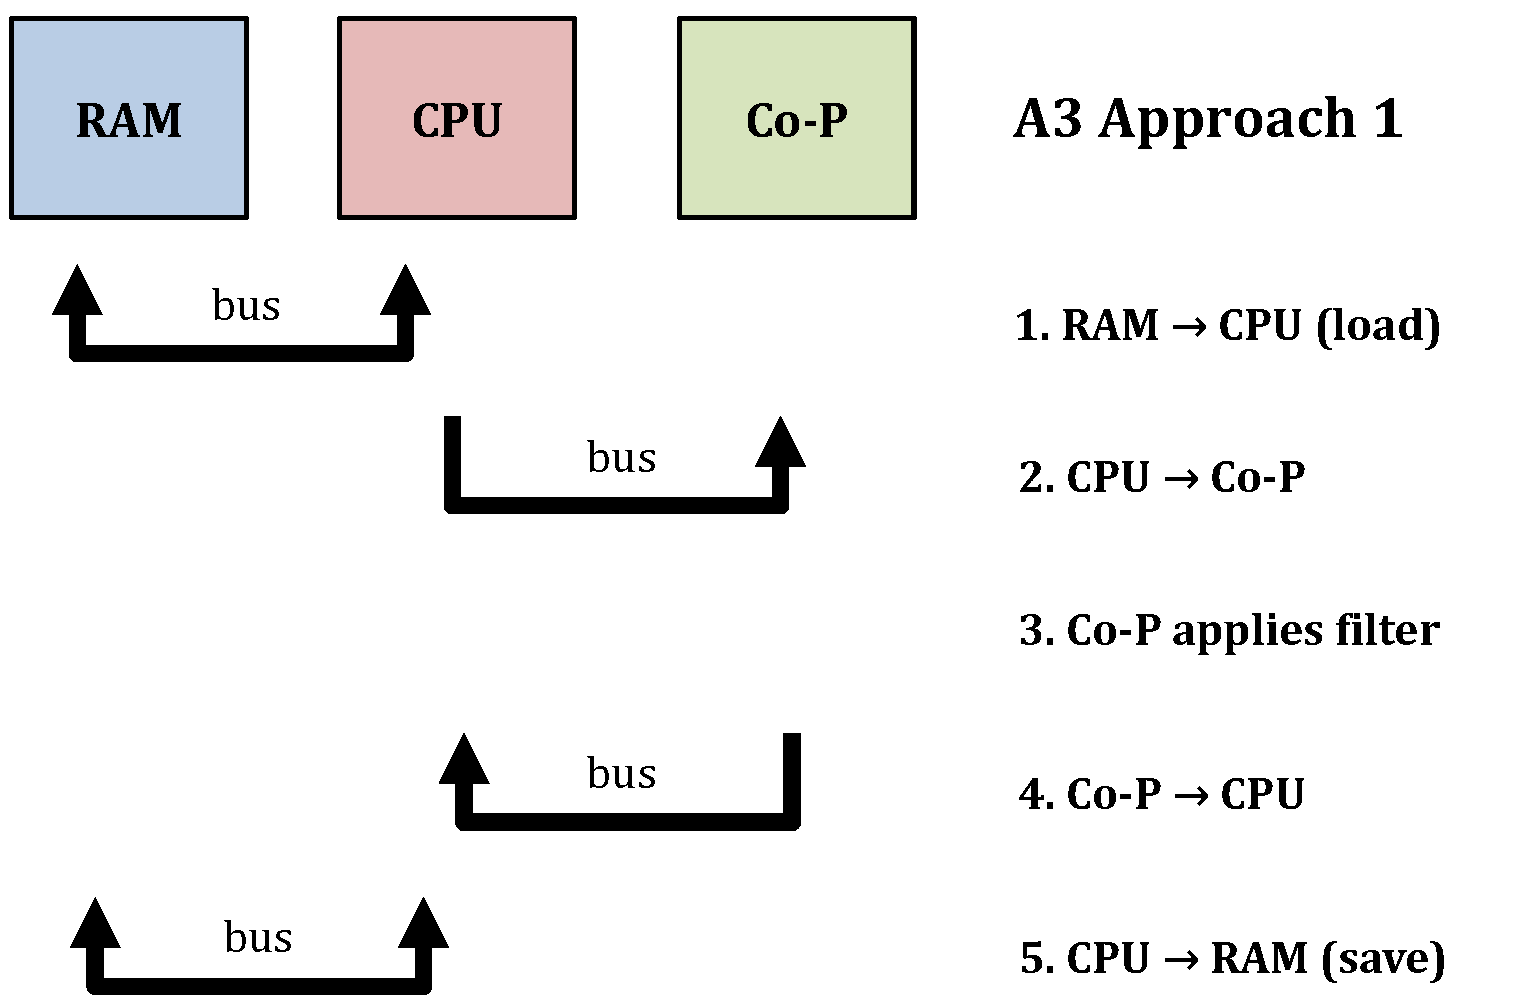
\includegraphics[width=0.75\textwidth]{2Implementation/fig/interaction1.pdf}
    \caption{Interaction pattern for approach 1 in Gezel. All communication between components happens through the bus. Arrows with two heads represent the bus waiting for a response.}
    \label{fig:interaction1}
\end{figure}

\textbf{Approach 2} requires fewer interactions between components, and most actions occurs in parallel. First CPU and Co-P swap values; Co-P receives a new data point to which it should apply the MWI filter, CPU receives the last filtered data point. \\

CPU saves its current filtered data point to RAM, and loads a new one. Loading and saving in RAM takes longer than applying the MWI filter, so Co-P eventually goes into idle mode waiting for CPU to reciprocate the handshake. This approach minimizes the interaction between Co-P and CPU.

\begin{figure}[H]
    \centering
    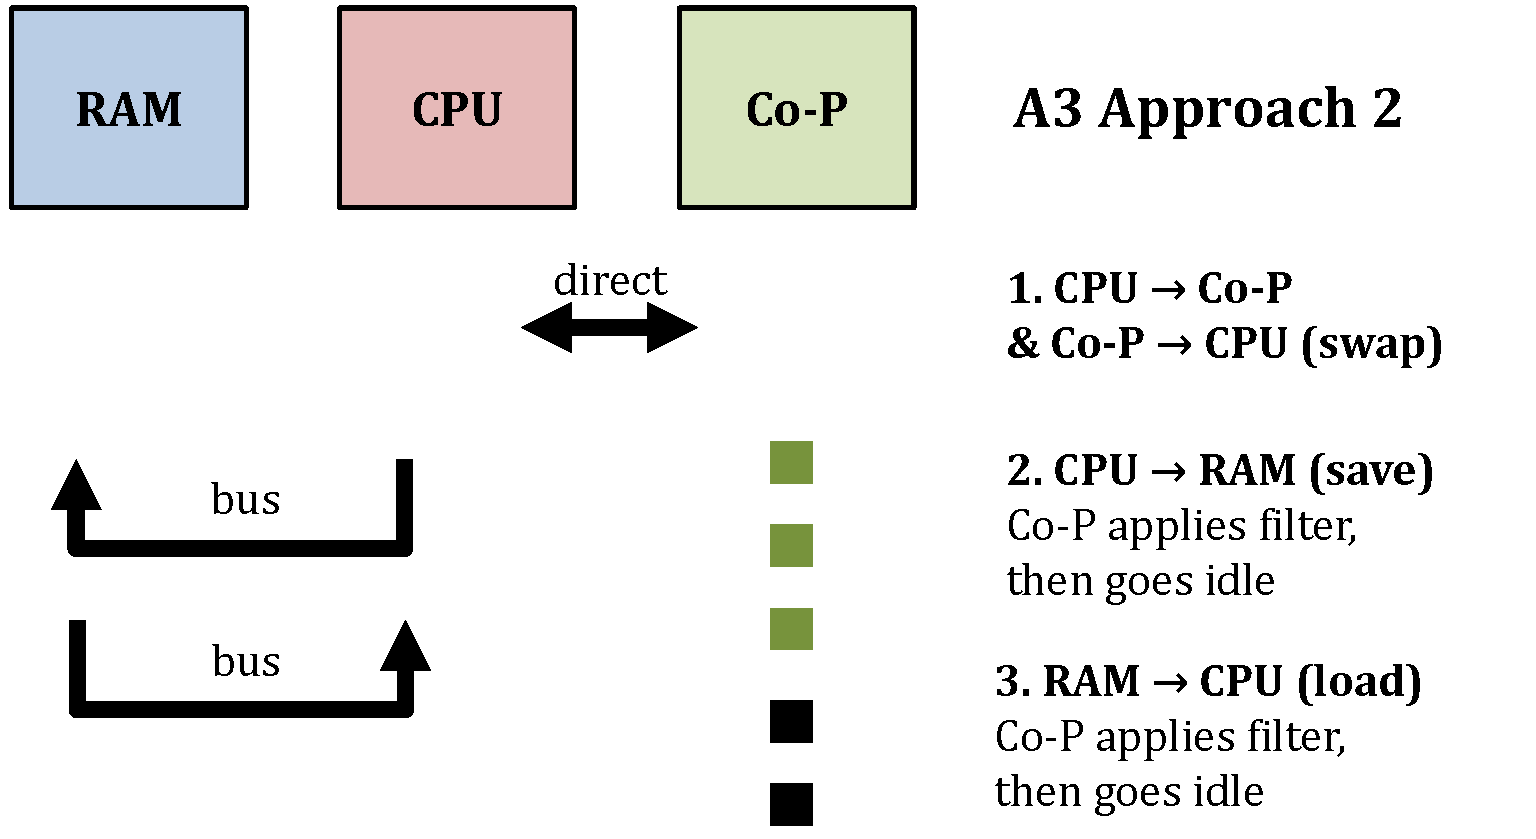
\includegraphics[width=0.75\textwidth]{2Implementation/fig/interaction2.pdf}
    \caption{Interaction pattern for approach 2 in Gezel. Communication between CPU and external memory happens through the bus. Communication between CPU and Co-P happens through a direct connection.}
    \label{fig:interaction2}
\end{figure}
